\documentclass[12pt,fleqn]{article}\usepackage{../../common}
\begin{document}
Çift Sarkaç (Double Pendulum)

En basit formunda çifte sarkaç $L_1,L_2$ uzunluğunda kütlesiz iki çubuk, iki
$m_1,m_2$ kütlesindeki iki topu birleştirir ve sallandırır. Eğer $m_1$'in
olduğu kordinatları $x_1,y_1$, $m_2$ kütlesini $x_2,y_2$ ile belirtirsek,

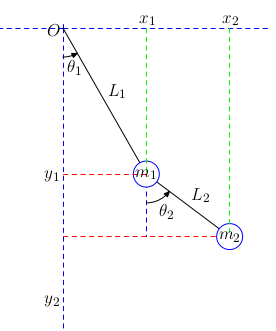
\includegraphics[width=15em]{phy_dblpend_01.png}

$$
x_1 = L_1 \sin\theta_1
$$

$$
y_1 = - L_1 \cos\theta_1
$$

$$
x_2 = L_2  (\sin\theta_1 +  \sin\theta_2) 
$$

$$
y_2 = -L_2  (\cos\theta_1 + \cos \theta_2)
$$

Mesela $y_1$ için $- L_1 \cos\theta_1$ olmasının sebebi kordinat
bakımından aşağı doğru gidiyor olmamız. 

Bu sistemi şurada şu kuvvet, artı şurada şu kuvvet, şurada hareket şeklinde
modelleyebilirdik, fakat daha kolay bir yöntem sistemin Lagrangian'inini
hesaplamak ve onun optimalliği üzerinden Euler-Lagrange denklemlerini
kullanıp sistemın formüllerinin burada dökülmesini sağlamak. 

Sistemin Lagrangian'ını hesaplayacağız, $L = K - P$. 

Kinetik enerji $K$ hesabını $\frac{1}{2} m v^2$ üzerinden yapabiliriz, ve
$v$ bileşenlerini yatay, dikey üzerinden düşünürsek,
$v = \sqrt{v_x^2 + v_y^2}$ ya da $v^2 = v_x^2 + v_y^2$, ve üstteki örnekte
hız kütle \#1 için $\dot{x}_1$ kütle \#2 için $\dot{x}_2$. O zaman

$$
K = \frac{1}{2} m_1 ( \dot{x}_1 ^2 + \dot{y}_1 ^2 )  + m_2 ( \dot{x}_2 ^2 + \dot{y}_2 ^2 ) 
$$

Açmak için $\dot{x}_1, \dot{x}_2$, vs bulunmalı, üstteki $x_1$'in $t$
üzerinden türevini almak lazım yani, hepsini yapinca,

$$
\dot{x}_1 = L_1 \cos^2(\theta_1)\dot{\theta_1}
$$

$$
\dot{y}_1 = L_1 \sin(\theta_1)\dot{\theta_1}
$$

$$
\dot{x}_2 = L_1 \cos(\theta_1)\dot{\theta}_1 + L_2 \cos (\theta_2)\dot{\theta}_2
$$

$$
\dot{y}_2 = L_1 \sin(\theta_1)\dot{\theta}_1 + L_2 \sin(\theta_2)\dot{\theta}_2
$$

$$
K = 
1/2 m_1 \dot{\theta}_1^2 L_1^2 + 
1/2 m_2 [
 \dot{\theta}_1^2 L_1^2 + \dot{\theta}_2^2 L_2^2  + 
 2 \dot{\theta}_1^2 L_1 \dot{\theta}_1L_2\cos(\theta_1 - \theta_2)]
$$

Potansiyel enerjiye gelelim, tek sarkaçtan $m g h$ formülü en yüksek
noktada en fazla potansiyel enerji verir. Bir kordinat sisteminde kütle
\#1'ın sabitlendiği noktaya orijin dedik, o zaman en alt noktada enerji en
azdir. Fakat mesela $L_1$ negatif, pozitifsel durumu bunları idare eder
zaten, biz direk formülü yazarsak,

$$
P = m g y_1 + m g y_2
$$

Sadece dikey kordinat kullanıldı çünkü potansiyel enerji üzerinde tek
etkili olan dikey kordinattır. 

$$
P = -m_1 g L_1 \cos(\theta_1) - m_2 g (L_1 \cos(\theta_1) + L_2 \cos(\theta_2))
$$

Lagrangian $L = K - P$'yi elde etmek icin 

$$
L = 
\frac{1}{2} m_1 (\dot{\theta}_1 L_1)^2 + 
\frac{1}{2} m_2 [(\dot{\theta}_1L_1)^2 + 
(\dot{\theta}_2 L_2 )^2  +  ..
$$
$$
 2 \dot{\theta}_1^2 L_1 \dot{\theta}_1L_2\cos(\theta_1 - \theta_2)] -
[-(m_1+m_2) g L_1 \cos(\theta_1) - m_2 L_2 g \cos(\theta_2)]
$$

Basitleştirince

$$
L = \frac{1}{2} (m_1 + m_2) L_1^2 \dot{\theta}_1^2 + 
\frac{1}{2} m_2 L_2^2 \dot{\theta}_2^2 + 
m_2 L_1 L_2 \dot{\theta}_1\dot{\theta}_2 \cos(\theta_1-\theta_2) + ..
$$
$$
(m_1 + m_2) g L_1 \cos(\theta_1) + m_2 L_2  g \cos(\theta_2)
$$

Bu sistemden bir fiziksel sistemi üretmek istiyorsam $L$'yi minimize edecek
fonksiyonları elde etmem lazım. Burada bir değişimsel calculus problemi
var, yani Euler-Lagrange denklemlerine bakabilirim. 

$$
\frac{\ud}{\ud t} \left(
\frac{\partial L}{\partial \dot{\theta}} 
\right) -
\frac{\partial L}{\partial \theta} = 0
$$

Her $\theta_1,\theta_2$ için üstteki denklemi kullanacağım, ve elde ettiğim
formüller bu sistemin dinamik formülleri olacaklar. 

$\theta_1$ için

$$
\frac{\partial L}{\partial \theta_1} = 
-L_1 g (m_1 + m_2) \sin(\theta_1) - m_2 L_1 L_2 \dot{\theta}_1\dot{\theta_2}\sin(\theta_1-\theta_2)
$$

$$
\frac{\partial L}{\partial \dot{\theta}_1} = 
(m_1 + m_2) L_1^2 \dot{\theta}_1 + m_2 L_1 L_2 \dot{\theta}_2 \cos(\theta_1- \theta_2)
$$
 
$$
\frac{\ud }{\ud t} \left(
\frac{\partial L}{\partial \dot{\theta}_1} \right) = 
(m_1 + m_2) L_1^2 \ddot{\theta}_1 + m_2 L_1 L_2 \ddot{\theta}_2 \cos(\theta_1-\theta_2)-
m_2 L_1 L_2 \dot{\theta}_2 \sin(\theta_1-\theta_2)(\dot{\theta}_1 - \dot{\theta}_2)
$$

Üsttekileri bir araya koyarsak,

$$
\Rightarrow (m_1 + m_2) L_1^2 \ddot{\theta}_1 + 
m_2L_1 L_2 \ddot{\theta}_2 \cos(\theta_1-\theta_2)-
$$
$$
m_2 L_1 L_2 \dot{\theta}_2 \sin(\theta_1-\theta_2)(\dot{\theta}_1 - \dot{\theta}_2) +
g L_1 (m_1 + m_2) \sin(\theta_1) + 
m_2 L_1 L_2 \dot{\theta}_1\dot{\theta_2}\sin(\theta_1-\theta_2)=0
$$

$$
\Rightarrow (m_1 + m_2) L_1^2 \ddot{\theta}_1 + 
m_2 L_1 L_2 \ddot{\theta}_2 \cos(\theta_1-\theta_2) +
g L_1 (m_1 + m_2) \sin(\theta_1) + 
$$
$$
m_2 L_1 L_2\dot{\theta}_2 \sin(\theta_1-\theta_2) \left[ (\dot{\theta}_1 - \dot{\theta}_1 + \dot{\theta}_2)  \right]
=0
$$

$$
\frac{\ud}{\ud t} \left(
\frac{\partial L}{\partial \dot{\theta_1}} 
\right) - \frac{\partial L}{\partial \theta_1} =  
(m_1 + m_2) L_1^2 \ddot{\theta}_1 + 
m_2 L_1 L_2 \ddot{\theta}_2 \cos(\theta_1-\theta_2) +
g L_1 (m_1 + m_2) \sin(\theta_1) + 
$$
$$
m_2 L_1 L_2\dot{\theta}_2^2 \sin(\theta_1-\theta_2) 
=0
$$

Basitleştirip $\ddot{\theta}_1$ için çözelim,

$$
\ddot{\theta}_1 = \frac{
-m_2 L_2 \ddot{\theta}_2 \cos (\theta_1-\theta_2) - 
m_2 L_2 \dot{\theta}_2^2 \sin(\theta_1 - \theta_2) - (m_1 + m_2) g \sin(\theta_1)
}
{(m_1 + m_2) L_1 }
\mlabel{2}
$$

$\theta_2$ için

$$
\frac{\partial L}{\partial \theta_2} = 
m_2 L_1 L_2 \dot{\theta}_1 \dot{\theta}_2 \sin(\theta_1 - \theta_2) - 
L_2 m_2 g \sin(\theta_2)
$$

$$
\frac{\partial L}{\partial \dot{\theta}_2 } = 
m_2 L_2^2 \dot{\theta}_2 + m_2 L_1 L_2 \dot{\theta}_1 \cos(\theta_1 - \theta_2)
$$

$$
\frac{\ud}{\ud t} \left(\frac{\partial L}{\partial \dot{\theta_2}}  \right) =
m_2 L_2^2 \ddot{\theta}_2 + m_2 L_1 L_2 \ddot{\theta}_1 \cos(\theta_1 - \theta_2)
- m_2 L_1 L_2 \dot{\theta}_1 \sin(\theta_1 - \theta_2)(\dot{\theta}_1 - \dot{\theta}_2)
$$

E-L denklemine sokunca

$$
\frac{\ud}{\ud t} \left(
\frac{\partial L}{\partial \dot{\theta_2}} 
\right) - \frac{\partial L}{\partial \theta_2} =  
L_2 \ddot{\theta}_2 + L_1 \ddot{\theta}_1 \cos(\theta_1 - \theta_2) - 
L_1 \dot{\theta}_1^2 \sin(\theta_1 - \theta_2) + g \sin (\theta_2) = 0
$$

Aynı şekilde basitleştirip $\ddot{\theta}_2$ için çözelim,

$$
\ddot{\theta}_2 = 
\frac{
-L_1 \ddot{\theta}_1 \cos(\theta_1-\theta_2) + 
L_1 \dot{\theta}_1^2\sin(\theta_1-\theta_2) - 
g \sin(\theta_2)
}
{L_2}
\mlabel{1}
$$

(1) ve (2) formüllerine bakarsak elimde $\ddot{\theta}_2$'ye dayanan bir
$\ddot{\theta}_1$ formülü, $\ddot{\theta}_1$'e dayanan bir
$\ddot{\theta}_2$ formülü var. Bu formülleri kullanarak içinde aynı anda
$\ddot{\theta}_1$ ya da $\ddot{\theta}_2$ içermeyen (yani her denklem ya
sadece $\ddot{\theta}_1$ ya da sadece $\ddot{\theta}_2$ içerecek) iki tane
yeni formül üretebilirim.

Eğer (1)'i (2) içine sokarsak, 

$$
\ddot{\theta}_1 (m_1 + m_2) L_1 = -m_2 
\big[-L_1\ddot{\theta}_1 \cos(\theta_1-\theta_2) + 
 L_1\dot{\theta}_1^2 \sin(\theta_1-\theta_2) -
 g \sin(\theta_2) \big] \cos(\theta_1-\theta_2)- 
$$
$$
m_2 L_2 \dot{\theta}_2^2 \sin(\theta_1-\theta_2)- 
(m_1 + m_2) g \sin(\theta_1)
$$

İçinde $\ddot{\theta}_1$ olan tüm terimleri eşitliğin sol tarafına taşırsam,

$$
\ddot{\theta}_1 [L_1 (m_1 + m2) - m_2 L_1 \cos^2(\theta_1-\theta_2)] =
-m_2 L_1 \dot{\theta}_1^2 \sin(\theta_1-\theta_2) \cos(\theta_1-\theta_2) + 
g m_2 \sin(\theta_2) \cos(\theta_1-\theta_2) - 
$$
$$
m_2 L_2 \dot{\theta}_2^2 \sin(\theta_1-\theta_2) - 
(m_1 + m_2) g \sin(\theta_1)
$$

$\ddot{\theta}$ için çözersem, 

$$
 -m_2 L_1 \dot{\theta}_1^2 \sin(\theta_1-\theta_2)\cos(\theta_1-\theta_2) + 
$$
$$
\ddot{\theta}_1 = 
\frac{ g m_2 \sin(\theta_2)\cos(\theta_1-\theta_2) -
m_2 L_2 \dot{\theta}_2^2 \sin(\theta_1-\theta_2) - (m_1+m_2)g\sin(\theta_1)
}
{L_1 (m_1+m_2)-m_2L_1\cos^2(\theta_1-\theta_2)}
\mlabel{3}
$$

Dikkat: Bölünen çok kalabalık, o iki satır bölünendeki değerleri
gösteriyor. 

Aynı şekilde $\ddot{\theta}_2$ için işlem yapınca, 

$$
m_2 L_2 \dot{\theta}_2^2 \sin(\theta_1-\theta_2)\cos(\theta_1-\theta_2) + 
$$
$$
\ddot{\theta}_2 = 
\frac{ 
g \sin(\theta_1) \cos(\theta_1-\theta_2)(m_1+m_2) + 
L_1 \dot{\theta}_1^2 \sin(\theta_1-\theta_2)(m_1+m_2) - g\sin(\theta_2) (m_1+m_2)
}
{L_2 (m_1+m_2) - m_2 L_2 \cos^2 (\theta_1-\theta_2)}
\mlabel{4}
$$

Artık elimde iki tane ikinci dereceden diferansiyel denklem var. Bu
denklemleri birinci derece diferansiyel denkleme çevirebilirim. Ufak bir
değişken değimi numarası kullanırsam, 

$$
z_1 = \theta_1, \quad
z_2 = \theta_2, \quad
z_3 = \dot{\theta}_1, \quad
z_4 = \dot{\theta}_2
$$

Bu değişkenlerin türevini alırsam, 

$$
\dot{z}_1 = \dot{\theta}_1, \quad
\dot{z}_2 = \dot{\theta}_2, \quad
\dot{z}_3 = \ddot{\theta}_1, \quad
\dot{z}_4 = \ddot{\theta}_1
$$

Böylece dört yeni diferansiyel denklem yarattık. (3), (4) denklemlerinde
$\theta_1$ yerine $z_1$, $\dot{\theta}_2$ yerine $z_4$, $\dot{\theta}_1$
yerine $z_3$, vs. koyunca,

$$
\dot{z}_1 = \dot{\theta}_1
$$

$$
\dot{z}_2 = \dot{\theta}_2
$$

$$
 -m_2 L_1 z_4^2 \sin(z_1-z_2)\cos(z_1-z_2) + 
$$
$$
\dot{z}_3 = 
\frac{ g m_2 \sin(z_2)\cos(z_1-z_2) -
m_2 L_2 z_4^2 \sin(z_1-z_2) - (m_1+m_2)g\sin(z_1)
}
{L_1 (m_1+m_2)-m_2L_1\cos^2(z_1-z_2)}
$$

$$
m_2 L_2 z_4^2 \sin(z_1-z_2)\cos(z_1-z_2) + 
$$
$$
\dot{z}_4 = 
\frac{ 
g \sin(z_1) \cos(z_1-z_2)(m_1+m_2) + 
L_1 z_4^2 \sin(z_1-z_2)(m_1+m_2) - g\sin(z_2) (m_1+m_2)
}
{L_2 (m_1+m_2) - m_2 L_2 \cos^2 (z_1-z_2)}
$$

Bu ODE sistemini sayısal olarak çözebiliriz. Başlangıç açılarını
$\theta_1,\theta_2$ için $\pi/4$ olarak seçtik, sarkaç sağ taraftan
başlayacak, ve sallanacak. 

\begin{minted}[fontsize=\footnotesize]{python}
from matplotlib.patches import Circle
import matplotlib.pyplot as plt
from numpy import cos, sin
from scipy.integrate.odepack import odeint

m1=1.0; m2=1.0; L1=1.0; L2=1.0
g=9.8

def f(z, t):
    z1, z2, z3, z4 = z
    tmp1 = (-m2*L1*z4**2*sin(z1-z2)*cos(z1-z2) + g*m2*sin(z2)*cos(z1-z2) - \
            m2*L2*z4**2*sin(z1-z2) - (m1+m2)*g*sin(z1)) \
            /(L1*(m1+m2)-m2*L1*cos(z1-z2)**2);
    tmp2 = (m2 * L2 * (z4**2) *sin(z1-z2) * cos(z1-z2) + \
            g*sin(z1)*cos(z1-z2)*(m1+m2) + L1*(z4**2)*sin(z1-z2)*(m1+m2) - \
            g*sin(z2)*(m1+m2)) \
    / (L2*(m1+m2)-m2*L2*cos(z1-z2)**2)
    z = [ z3, z4, tmp1, tmp2 ]
    return z

z0 = np.array([np.pi/4, np.pi/4, 0.0, 0.0])
t = np.linspace(0, 10, 100)

z = odeint(f, z0, t)

x1=L1*sin(z[:,0])
y1=-L1*cos(z[:,0])
x2=L1*sin(z[:,0])+L2*sin(z[:,1])
y2=-L1*cos(z[:,0])-L2*cos(z[:,1])


def make_plot(fout,x1,y1,x2,y2):
    r = 0.05
    fig = plt.figure()
    ax = fig.add_subplot(111)
    ax.set_xlim(-2,2)
    ax.set_ylim(-2,2)
    plt.plot([0, x1, x2], [0, y1, y2], lw=2, c='k')
    c0 = Circle((0, 0), r/2, fc='k', zorder=10)
    c1 = Circle((x1, y1), r, fc='b', ec='b', zorder=10)
    c2 = Circle((x2, y2), r, fc='r', ec='r', zorder=10)
    ax.add_patch(c0)
    ax.add_patch(c1)
    ax.add_patch(c2)
    plt.savefig(fout)

for i in range(len(x1)):
    if i % 5 == 0: 
        make_plot('frames/img{:04d}.png'.format(i),x1[i],y1[i],x2[i],y2[i])
\end{minted}

Birkac ornek, 

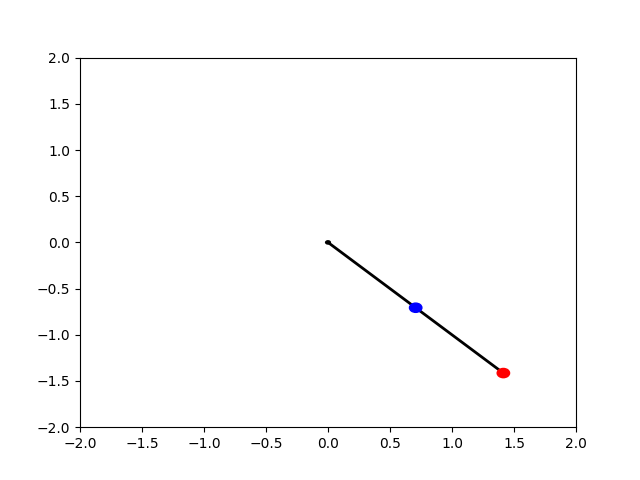
\includegraphics[width=12em]{frames/img0000.png}
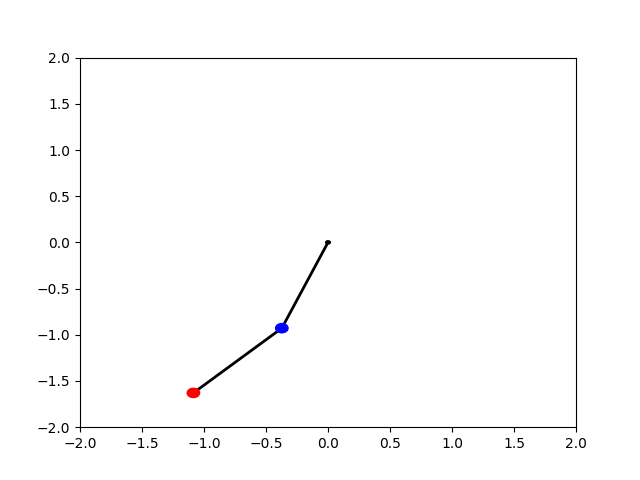
\includegraphics[width=12em]{frames/img0010.png}
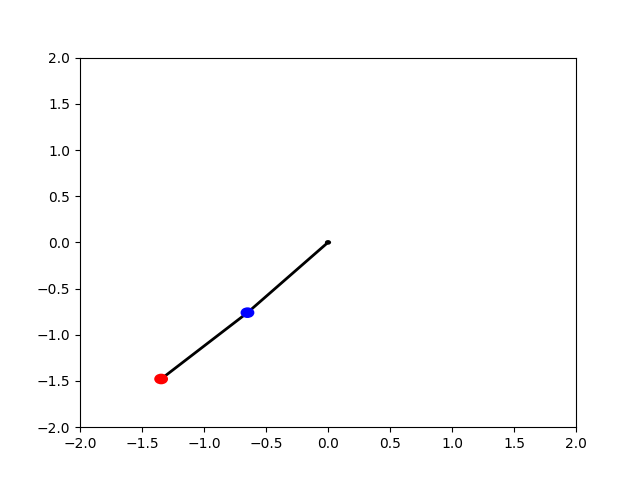
\includegraphics[width=12em]{frames/img0015.png}

Sistemin belli anlarda ``fotoğrafını çekip'' grafikledik, ve bu grafikleri
animasyon olarak birleştirirsek,

\begin{minted}[fontsize=\footnotesize]{python}
! convert -loop 0 -delay 100 frames/*.png frames/dblpend.gif
\end{minted}

Sonuçları [2]'de bulabiliriz. 

Kaynaklar

[1] Altic, \url{sophia.dtp.fmph.uniba.sk/~kovacik/doublePendulum.pdf}

[2] Bayramli, {\em Double Pendulum Animasyonu}, \url{https://raw.githubusercontent.com/burakbayramli/classnotes/master/phy/phy_050_cont4/frames/dblpend.gif}

[3] \url{http://galileo.phys.virginia.edu/education/outreach/8thgradesol/EnergyPendulum.htm}

[4] Altic, \url{https://mse.redwoods.edu/darnold/math55/DEproj/sp08/jaltic/ProjectTitleOnline.pdf}

\end{document}

